%!TEX program = xelatex
%http://tex.stackexchange.com/questions/148843/how-to-write-over-a-table

\documentclass[UTF8, adobefonts, oneside]{ctexbook} \newcommand{\whzkjk}{\kaishu}
%\documentclass[oneside]{book} \input{setupfonts}


\newcommand{\doctitle}{《中文》描红}
\newcommand{\docauthor}{Yunhui Fu}
\newcommand{\dockeywords}{{中文}{描红}}
\newcommand{\docsubject}{《中文》描红}

\usepackage{ifthen}
\usepackage{ifpdf}
\usepackage{ifxetex}
\usepackage{ifluatex}


\usepackage{amsfonts,amssymb}


\usepackage{color}
\usepackage[rgb]{xcolor}




\usepackage{tikz}
\usepackage{geometry}
%\geometry{margin = 2.1cm, papersize = {16cm, 13cm}}
\geometry{top=2cm, bottom=2cm, left=2cm, right=2cm,}
\pagestyle{empty}
\linespread{0.833333}

\makeatletter
\ExplSyntaxOn
\box_new:N \l_@@_grid_box % l means local
\coffin_new:N \l_@@_grid_coffin
\coffin_new:N \l_@@_charater_coffin
\int_const:Nn \c_@@_test_char { "4E00 }
\cs_new_protected_nopar:Npn \@@_update_grid_box:
  {
    \hbox_set:Nn \l_@@_grid_box
      { \XeTeXuseglyphmetrics = \c_zero \c_@@_test_char }
    \use:x
      {
        \@@_update_grid_box:nnn
          { \dim_use:N \box_wd:N \l_@@_grid_box } % width
          { \dim_use:N \box_ht:N \l_@@_grid_box } % height
          { \dim_use:N \box_dp:N \l_@@_grid_box } % depth
      }
    \coffin_attach:NnnNnnnn
      \l_@@_charater_coffin { hc } { vc }
      \l_@@_grid_coffin     { hc } { vc }
      { \c_zero_dim } { \c_zero_dim }
    \hbox_set:Nn \l_@@_grid_box
      {
        \coffin_typeset:Nnnnn \l_@@_charater_coffin
          { H } { l } { \c_zero_dim } { \c_zero_dim }
      }
    \box_set_wd:Nn \l_@@_grid_box { \c_zero_dim }
    \box_set_ht:Nn \l_@@_grid_box { \c_zero_dim }
    \box_set_dp:Nn \l_@@_grid_box { \c_zero_dim }
  }
\cs_new_protected_nopar:Npn \@@_update_grid_box:nnn #1#2#3
  {
    \hbox_set:Nn \l_@@_grid_box { }
    \box_set_wd:Nn \l_@@_grid_box {#1}
    \box_set_ht:Nn \l_@@_grid_box {#2}
    \box_set_dp:Nn \l_@@_grid_box {#3}
    \hcoffin_set:Nn \l_@@_charater_coffin { \box_use:N \l_@@_grid_box }
    \@@_draw_grid:nn {#1} { (#2) + (#3) }
  }
\cs_new_protected_nopar:Npn \@@_draw_grid:nn #1#2
  {
    \use:x
      {
        % 米字格
        %\@@_draw_grid:nnnn { \dim_eval:n {#1} } { \dim_eval:n {#2} }
          %{ \dim_eval:n { (#1) / 2 } } { \dim_eval:n { (#2) / 2 } }
        % 田字格
        \@@_draw_grid_tian:nnnn { \dim_eval:n {#1} } { \dim_eval:n {#2} }
          { \dim_eval:n { (#1) / 2 } } { \dim_eval:n { (#2) / 2 } }
        % 九宫格
        %\@@_draw_grid:nnnnnn { \dim_eval:n {#1} } { \dim_eval:n {#2} }
          %{ \dim_eval:n { (#1) / 3 } } { \dim_eval:n { (#2) / 3 } }
          %{ \dim_eval:n { (#1) * 2 / 3 } } { \dim_eval:n { (#2) * 2 / 3 } }
      }
  }
\cs_new_protected_nopar:Npn \@@_draw_grid:nnnn #1#2#3#4
  {
    \hcoffin_set:Nn \l_@@_grid_coffin
      {
        \begin{tikzpicture}
          \draw[help~lines, red] (0,#4) -- (#1,#4) (#3,0) -- (#3,#2);
          \draw[help~lines, red, dashed] (0,0) -- (#1,#2) (0,#2) -- (#1,0);
          \draw[help~lines, red, thick] (0,0) rectangle (#1,#2);
        \end{tikzpicture}
      }
  }
\cs_new_protected_nopar:Npn \@@_draw_grid_tian:nnnn #1#2#3#4
  {
    \hcoffin_set:Nn \l_@@_grid_coffin
      {
        \begin{tikzpicture}
          \draw[help~lines, red, dashed] (0,#4) -- (#1,#4) (#3,0) -- (#3,#2);
          \draw[help~lines, red, thick] (0,0) rectangle (#1,#2);
        \end{tikzpicture}
      }
  }
\cs_new_protected_nopar:Npn \@@_draw_grid:nnnnnn #1#2#3#4#5#6
  {
    \hcoffin_set:Nn \l_@@_grid_coffin
      {
        \begin{tikzpicture}
          \draw[help~lines, red, dashed] (0,#4) -- (#1,#4) (#3,0) -- (#3,#2) (0,#6) -- (#1,#6) (#5,0) -- (#5,#2);
          \draw[help~lines, red, thick] (0,0) rectangle (#1,#2);
        \end{tikzpicture}
      }
  }
\cs_new_protected_nopar:Npn \@@_grid_CJKsymbol:n
  { \box_use:N \l_@@_grid_box \@@_grid_CJKsymbol:n }
\cs_new_protected_nopar:Npn \@@_grid_CJKpunctsymbol:n
  { \box_use:N \l_@@_grid_box \@@_grid_CJKpunctsymbol:n }
\keys_define:nn { @@ }
  {
    format .tl_set:N  = \l_@@_formal_tl ,
    format .initial:n = { \normalfont }
  }
\cs_new_protected:Npn \@@_active_grid:n #1
  {
    \xeCJKsetup{PunctStyle=plain,CJKglue=\allowbreak,AllowBreakBetweenPuncts}
    \keys_set:nn { @@ } {#1}
    \tl_use:N \l_@@_formal_tl
    \@@_update_grid_box:
    \xeCJK_swap_cs:NN \CJKsymbol \@@_grid_CJKsymbol:n
    \xeCJK_swap_cs:NN \CJKpunctsymbol \@@_grid_CJKpunctsymbol:n
    \__xeCJK_add_to_shipout:n
      {
        \xeCJK_swap_cs:NN \CJKsymbol \@@_grid_CJKsymbol:n
        \xeCJK_swap_cs:NN \CJKpunctsymbol \@@_grid_CJKpunctsymbol:n
      }
  }
\NewDocumentCommand \CJKgrid { +O { } +m }
  { \group_begin: \@@_active_grid:n {#1} #2 \relax \group_end: }
\NewDocumentEnvironment { CJKGrid } { +O { } }
  { \@@_active_grid:n {#1} } { \par }
\ExplSyntaxOff

%\newcommand\miline[1]{\CJKgrid{\kaishu #1\color{gray!20} \whzkbk #1 #1 #1\color{white} #1 #1 #1 #1} \newline }



%\newcommand\milinetwo[3]{\CJKgrid{\kaishu #1\color{gray!20} #1\color{white} #1 #2\color{gray!20} #1\color{white} #2 #2 #2 #3 #3 #3 #3 } \newline }
\newcommand\milinetwo[3]{\CJKgrid{\kaishu #1\color{gray!20}\whzkjk #1\color{white}\kaishu #1 #2\color{gray!20}\whzkjk #1\color{white}\kaishu #2 #2 #2 #3 #3 #3 #3 } }

\newcommand\miline[1]{\milinetwo{#1}{厂}{水}}

%\newcommand\miline[1]{\CJKgrid{\kaishu #1\color{gray!20} #1\color{white} #1 #1\color{gray!20} #1\color{white} #1 #1 #1 #1 #1 #1 #1 } \newline }




\ifxetex % xelatex
\else
    %The cmap package is intended to make the PDF files generated by pdflatex "searchable and copyable" in acrobat reader and other compliant PDF viewers.
    \usepackage{cmap}%
\fi
% ============================================
% Check for PDFLaTeX/LaTeX
% ============================================
\newcommand{\outengine}{xetex}
\newif\ifpdf
\ifx\pdfoutput\undefined
  \pdffalse % we are not running PDFLaTeX
  \ifxetex
    \renewcommand{\outengine}{xetex}
  \else
    \renewcommand{\outengine}{dvipdfmx}
  \fi
\else
  \pdfoutput=1 % we are running PDFLaTeX
  \pdftrue
  \usepackage{thumbpdf}
  \renewcommand{\outengine}{pdftex}
  \pdfcompresslevel=9
\fi
\usepackage[\outengine,
    bookmarksnumbered, %dvipdfmx
    %% unicode, %% 不能有unicode选项,否则bookmark会是乱码
    colorlinks=true,
    citecolor=red,
    urlcolor=blue,        % \href{...}{...} external (URL)
    filecolor=red,      % \href{...} local file
    linkcolor=black, % \ref{...} and \pageref{...}
    breaklinks,
    pdftitle={\doctitle},
    pdfauthor={\docauthor},
    pdfsubject={\docsubject},
    pdfkeywords={\dockeywords},
    pdfproducer={Latex with hyperref},
    pdfcreator={pdflatex},
    %%pdfadjustspacing=1,
    pdfborder=1,
    pdfpagemode=UseNone,
    pagebackref,
    bookmarksopen=true]{hyperref}

% --------------------------------------------
% Load graphicx package with pdf if needed 
% --------------------------------------------
\ifxetex    % xelatex
    \usepackage{graphicx}
\else
    \ifpdf
        \usepackage[pdftex]{graphicx}
        \pdfcompresslevel=9
    \else
        \usepackage{graphicx} % \usepackage[dvipdfm]{graphicx}
    \fi
\fi



\title{\doctitle}

\begin{document}

\setlength{\parindent}{0pt}
%\Huge


\chapter*{使用说明}
\normalsize


%\usepackage{contour}
%\contour{black}{\textcolor{white}{低}}


对于小学低年级学生,直接对照字范(例字)学写汉字,一般是比较困难的。所以,在小学生的字帖里紧跟着字范,就会有一个或多个颜色较浅的字范供小孩子描摹(俗称“描红”)。但是从养成正确的汉字学写方法和提高学习效率角度考虑,描红的汉字不宜安排过多。有的孩子借助描红本学写汉字,养成了一种不当的学习习惯——看一笔写一笔,再看一笔再写一笔,结果要花上很多次练习机会才能完整地记住一个字的写法。


习字方法是:看字范(第一格),并借助对接下来的那个供描红的字范(第二格)的描摹,记住这个字的笔画、笔顺、间架结构以及诸笔画在田字格里的位置;然后,试着一气呵成临写出这个汉字(第三格),写好之后,将自己写的与字范进行比较,修正自己对字结构的记忆和理解;再一气呵试着临写一个(第四格),这个字往往写得还不如前一个,但这个字的结构开始内化在孩子的心里;为了让孩子有一个复习、对比和校正的机会,第五格最好是一个供描红的字,孩子可以选择描摹,也可以跳到下一个空白的田字格,继续临写。一般来说,正常的孩子在认真的状态下学习一个生字,经过1~2次描摹再加2~3次临写,基本上就能够掌握这个字的书写了。当然,如果要熟练和写得好看,还需要日后的练习。但是,为了让孩子早日习惯于在空白纸上写字,我建议把接下来的格子里的十字线去掉,改田字格为口字格,让孩子有机会摆脱田字格在空格里试写汉字。

与汉字识写规律对应,田字格这样设计:

\begin{itemize}
  \item 第1格:字范(例字)
  \item 第2格:描红(记忆性描摹)
  \item 第3-4格:空白田字格(一气呵成的临写)
  \item 第5格:描红(理解性描摹)
  \item 第6-7格:空白田字格(一气呵成的书写)
  \item 第8-12格:空白口字格(深入练习的书写)
\end{itemize}


\chapter{万能习字帖}
\normalsize

这个字根表包含90多个成字字根,全部是五笔字130多个字根里的汉字。五笔使用这些字根及偏旁部首,可处理 GB 2312-80 汉字集中的6763个汉字。
掌握了这写字根,识写字就相对简单了。看一下“激”字,就知道就这个字是由“三点水、一个白、一个方,一个反文旁”构成的,写一两遍就行了。也不必字字都默,能够说出字的结构就行。说不出的再看一下,练习一下就行了。如果孩子在上学之前有长期的亲子阅读经历,对许多汉字已经大致认识的情况下,快速有效识写汉字的一个法门,就是先准确地识写五笔字根表里的这90多个成字字根!


\begin{figure}[ht]\centering
  %\includegraphics[height=0.75\textheight]{figures/freq1.png}
  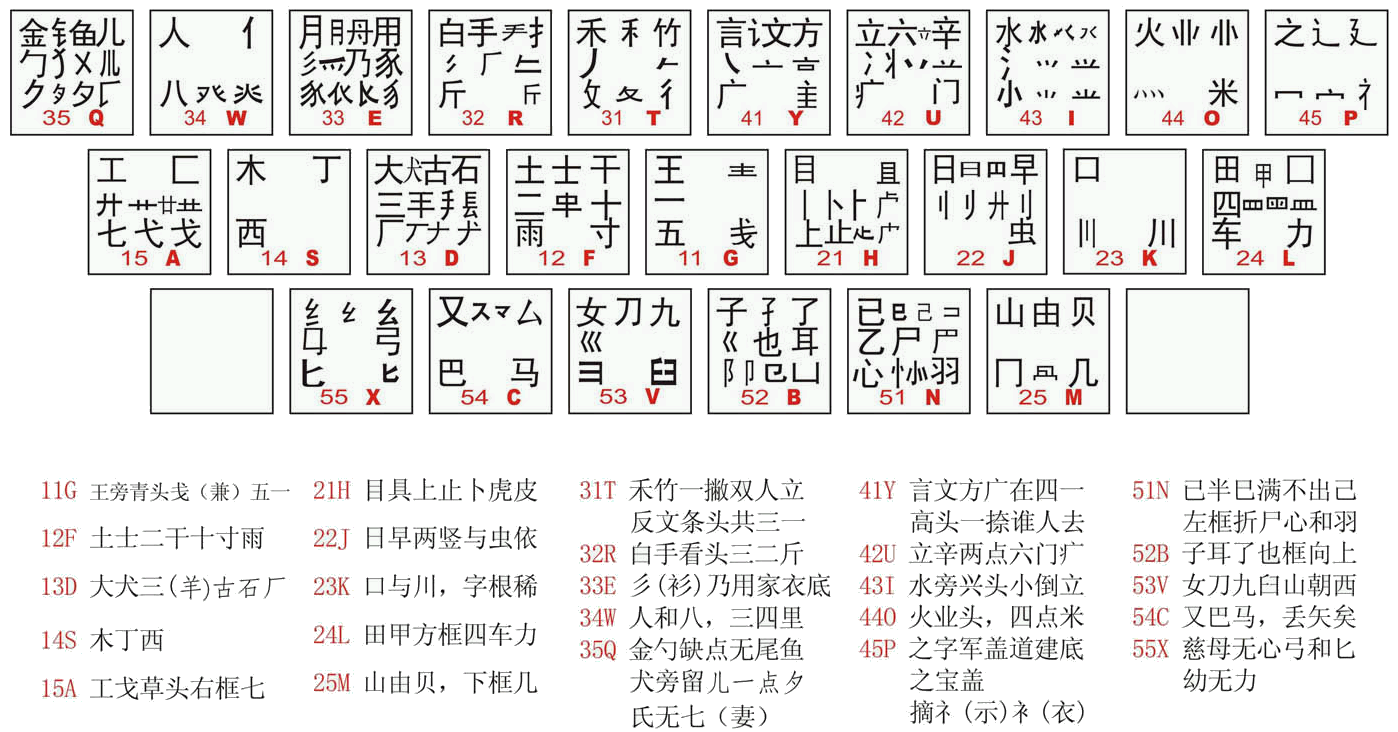
\includegraphics[width=0.8\textwidth]{figures/wubi86}
  \caption{五笔输入法字根表86版} \label{fig:wubi}
\end{figure}

%1区横起笔 11G 王旁青头戋(兼)五一 12F 土士二干十寸雨 13D 大犬三(羊)古石厂 14S 木丁西 15A 工戈草头右框七
%2区竖起笔 21H 目具上止卜虎皮 22J 日早两竖与虫依 23K 口与川,字根稀 24L 田甲方框四车力 25M 山由贝,下框几
%3区撇起笔 31T 禾竹一撇双人立,反文条头共三一 32R 白手看头三二斤 33E 月彡(衫)乃用家衣底 34W 人和八,三四里 35Q 金勺缺点无尾鱼,犬旁留儿一点夕,氏无七(妻)
%4区点起笔 41Y 言文方广在四一,高头一捺谁人去 42U 立辛两点六门疒(病) 43I 水旁兴头小倒立 44O 火业头,四点米 45P 之字军盖道建底,摘礻(示)衤(衣)
%5区折起笔 51N 已半巳满不出己,左框折尸心和羽 52B 子耳了也框向上 53V 女刀九臼山朝西 54C 又巴马,丢矢矣 55X 慈母无心弓和匕,幼无力


%\section{偏旁部首}
%\zihao{0}

%01画: 丨 亅 丿 乛 一 乙 丶
%\miline{丨}
%\miline{亅}
%\miline{丿}
%\miline{乛}
%\miline{一}
%\miline{乙}
%\miline{丶}

%02画: 八 勹 匕 冫 卜 厂 刀 刂 儿 二 匚 丷 几 卩 冂 力 冖 凵 人 亻 入 十 厶 亠 讠 廴 又
%\miline{八}
%\miline{勹}
%\miline{匕}
%\miline{冫}
%\miline{卜}
%\miline{厂}
%\miline{刀}
%\miline{刂}
%\miline{儿}
%\miline{二}
%\miline{匚}
%\miline{丷}
%\miline{几}
%\miline{卩}
%\miline{冂}
%\miline{力}
%\miline{冖}
%\miline{凵}
%\miline{人}
%\miline{亻}
%\miline{入}
%\miline{十}
%\miline{厶}
%\miline{亠}
%\miline{讠}
%\miline{廴}
%\miline{又}

%03画:干 艹 屮 彳 巛 川 辶 寸 大 飞 阝彑 工 弓 廾 广 己 彐 巾 口 马 门 宀 女 犭 山 彡 尸 饣 士 扌 氵 纟 巳 土 囗 兀 夕 小 忄 幺 弋 尢 夂 子
%04画: 贝 比 灬 长 车 歹 斗 厄 方 风 父 戈 卝 户 火 旡 见 斤 耂 毛 木 牛 牜 爿 片 攴 攵 气 欠 犬 日 氏 礻 手 殳 水 瓦 王 韦 文 无 毋 心 穴 牙 爻 曰 月 爫 支 止 爪 车
%05画: 白 癶 甘 瓜 禾 钅 立 龙 矛 皿 母 目 疒 鸟 皮 生 石 矢 示 罒 田 玄 疋 业 衤 用 玉
%06画: 臣 虫 而 耳 缶 艮 虍 臼 老 耒 米 糸 齐 肉 色 舌 糹 网 西 覀 行 血 羊 页 衣 羽 聿 至 舟 竹 自
%07画: 辰 赤 辵 豆 谷 龟 角 里 卤 麦 身 豕 辛 言 邑 酉 鱼 豸 走 足
%08画: 采 齿 非 阜 金 隶 黾 青 鱼 雨 隹 釒
%09画: 革 骨 鬼 韭 面 食(飠) 首 香 音
%10画: 髟 高 鬲 鬯 鬥 馬
%11画: 黄 鹿 麻 鹵 麥 鳥 魚
%12画: 鼎 黑 黽 黍 黹
%13画: 鼓 鼠 裏
%14画: 鼻 齊
%17画: 龠 齒 龍






%笔画数为一的部首:

    %丨
    %亅
    %丿
    %乛
    %一
    %乙
    %乚
    %丶

%笔画数为二的部首:

    %八
    %勹
    %匕
    %冫
    %卜
    %厂
    %刀
    %刂
    %儿
    %二
    %匚
    %阝
    %丷
    %几
    %卩
    %冂
    %力
    %冖
    %凵
    %人
    %亻
    %入
    %十
    %厶
    %亠
    %匸
    %讠
    %廴
    %又

%笔画数为三的部首:

    %艹
    %屮
    %彳
    %巛
    %川
    %辶
    %寸
    %大
    %飞
    %干
    %工
    %弓
    %廾
    %广
    %己
    %彐
    %彑
    %巾
    %口
    %马
    %门
    %宀
    %女
    %犭
    %山
    %彡
    %尸
    %饣
    %士
    %扌
    %氵
    %纟
    %巳
    %土
    %囗
    %兀
    %夕
    %小
    %忄
    %幺
    %弋
    %尢
    %夂
    %子

%笔画数为四的部首:

    %贝
    %比
    %灬
    %长
    %车
    %歹
    %斗
    %厄
    %方
    %风
    %父
    %戈
    %卝
    %户
    %火
    %旡
    %见
    %斤
    %耂
    %毛
    %木
    %肀
    %牛
    %牜
    %爿
    %片
    %攴
    %攵
    %气
    %欠
    %犬
    %日
    %氏
    %礻
    %手
    %殳
    %水
    %瓦
    %尣
    %王
    %韦
    %文
    %毋
    %心
    %牙
    %爻
    %曰
    %月
    %爫
    %支
    %止
    %爪

%笔画数为五的部首:

    %白
    %癶
    %歺
    %甘
    %瓜
    %禾
    %钅
    %立
    %龙
    %矛
    %皿
    %母
    %目
    %疒
    %鸟
    %皮
    %生
    %石
    %矢
    %示
    %罒
    %田
    %玄
    %穴
    %疋
    %业
    %衤
    %用
    %玉

%笔画数为六的部首:

    %耒
    %艸
    %臣
    %虫
    %而
    %耳
    %缶
    %艮
    %虍
    %臼
    %米
    %齐
    %肉
    %色
    %舌
    %覀
    %页
    %先
    %行
    %血
    %羊
    %聿
    %至
    %舟
    %衣
    %竹
    %自
    %羽
    %糸
    %糹

%笔画数为七的部首:

    %貝
    %采
    %镸
    %車
    %辰
    %赤
    %辵
    %豆
    %谷
    %見
    %角
    %克
    %里
    %卤
    %麦
    %身
    %豕
    %辛
    %言
    %邑
    %酉
    %豸
    %走
    %足

%笔画数为八的部首:

    %青
    %靑
    %雨
    %齿
    %長
    %非
    %阜
    %金
    %釒
    %隶
    %門
    %靣
    %飠
    %鱼
    %隹

%笔画数为九的部首:

    %風
    %革
    %骨
    %鬼
    %韭
    %面
    %首
    %韋
    %香
    %頁
    %音

%笔画数为十的部首:

    %髟
    %鬯
    %鬥
    %高
    %鬲
    %馬

%笔画数为十一的部首:

    %黄
    %鹵
    %鹿
    %麻
    %麥
    %鳥
    %魚

%笔画数为十二的部首:

    %鼎
    %黑
    %黽
    %黍
    %黹

%笔画数为十三的部首:

    %鼓
    %鼠

%笔画数为十四的部首:

    %鼻
    %齊

%笔画数为十五的部首:

    %齒
    %龍
    %龠



%\section{成字字根}
\zihao{0}

%\miline{我}
%\miline{喜}
%\miline{歡}
%\miline{寫}
%\miline{漢}
%\miline{字}

\miline{一}
\miline{二}
\miline{三}
\miline{十}
\miline{工}
\miline{干}
\miline{士}
\miline{土}
\miline{王}
\miline{上}
\miline{止}
\miline{廿}
\miline{厂}
\miline{川}
\miline{彳}
\miline{斤}
\miline{大}
\miline{八}
\miline{人}
\miline{木}
\miline{禾}
\miline{广}
\miline{文}
\miline{卜}
\miline{六}
\miline{米}
\miline{火}
\miline{犬}
\miline{立}
\miline{辛}
\miline{金}
\miline{耳}
\miline{口}
\miline{日}
\miline{曰}
\miline{目}
\miline{田}
\miline{甲}
\miline{由}
\miline{早}
\miline{贝}
\miline{白}
\miline{虫}
\miline{臼}
\miline{皿}
\miline{石}
\miline{言}
\miline{五}
\miline{尸}
\miline{又}
\miline{夕}
\miline{之}
\miline{山}
\miline{四}
\miline{西}
\miline{丁}
\miline{寸}
\miline{小}
\miline{水}
\miline{手}
\miline{子}
\miline{孑}
\miline{竹}
\miline{车}
\miline{幺}
\miline{女}
\miline{豕}
\miline{弋}
\miline{戈}
\miline{戋}
\miline{心}
\miline{刀}
\miline{方}
\miline{力}
\miline{门}
\miline{用}
\miline{雨}
\miline{羽}
\miline{月}
\miline{乙}
\miline{弓}
\miline{马}
\miline{乃}
\miline{因}




\chapter{中文1}

\zihao{0}

\section{第一单元}


%\miline{〇}
%\miline{零}
\miline{一}
\miline{二}
\miline{三}
\miline{四}
\miline{五}
\miline{六}
\miline{七}
\miline{八}
\miline{九}
\miline{十}
\miline{百}
\miline{千}
\miline{万}

\miline{又}
\miline{两}
\miline{水}
\miline{中}
\miline{不}
\miline{见}

\miline{人}
\miline{头}
\miline{目}
\miline{口}
\miline{耳}
\miline{手}
\miline{足}
\miline{大}
\miline{小}
\miline{多}
\miline{少}

\miline{我}
\miline{有}
\miline{左}
\miline{来}
\miline{右}
\miline{个}

\miline{日}
\miline{月}
\miline{山}
\miline{石}
\miline{田}
\miline{土}
\miline{水}
\miline{火}
\miline{木}
\miline{禾}

\section{第二单元}

\miline{上}
\miline{中}
\miline{下}
\miline{左}
\miline{右}
\miline{来}
\miline{去}
\miline{出}
\miline{入}
\miline{坐}
\miline{立}
\miline{走}

\miline{风}
\miline{云}
\miline{雨}
\miline{雪}
\miline{电}
\miline{天}
\miline{地}
\miline{春}
\miline{夏}
\miline{秋}
\miline{冬}

\miline{马}
\miline{牛}
\miline{羊}
\miline{鱼}
\miline{虫}
\miline{鸟}
\miline{草}
\miline{黄}
\miline{白}
\miline{黑}
\miline{绿}
\miline{红}
\miline{蓝}

\miline{自}
\miline{飞}
\miline{里}
\miline{爬}
\miline{游}
\miline{林}

\section{第三单元}

\miline{学}
\miline{生}
\miline{我}
\miline{是}
\miline{爱}
\miline{老}
\miline{师}
\miline{同}
\miline{文}
\miline{校}

\miline{家}
\miline{她}
\miline{你}
\miline{就}
\miline{像}
\miline{好}

\miline{开}
\miline{了}
\miline{真}
\miline{高}
\miline{兴}
\miline{车}
\miline{见}
\miline{说}
\miline{早}
\miline{你}
\miline{们}
\miline{好}

\miline{太}
\miline{阳}
\miline{对}
\miline{书}
\miline{包}
\miline{要}

\miline{的}
\miline{家}
\miline{这}
\miline{有}
\miline{爷}
\miline{奶}
\miline{爸}
\miline{妈}
\miline{和}

\miline{放}
\miline{回}
\miline{到}
\miline{给}
\miline{完}
\miline{把}

\section{第四单元}

\miline{花}
\miline{园}
\miline{门}
\miline{前}
\miline{个}
\miline{他}
\miline{后}
\miline{外}
\miline{年}
\miline{季}
\miline{儿}
\miline{看}

\miline{公}
\miline{朵}
\miline{可}
\miline{玫}
\miline{菊}
\miline{兰}

\miline{认}
\miline{方}
\miline{向}
\miline{面}
\miline{太}
\miline{阳}
\miline{东}
\miline{西}
\miline{北}
\miline{南}

\miline{象}
\miline{朋}
\miline{友}
\miline{猪}
\miline{起}

\miline{新}
\miline{到}
\miline{热}
\miline{闹}
\miline{穿}
\miline{衣}
\miline{戴}
\miline{帽}
\miline{祝}
\miline{身}
\miline{体}
\miline{习}

\miline{过}
\miline{团}
\miline{快}
\miline{乐}
\miline{平}
\miline{安}


\end{document}
